\documentclass{article}
\usepackage[T1]{fontenc}
\usepackage{lmodern}
\usepackage{graphicx}
\usepackage{amsmath,amssymb}
\usepackage[a4paper,margin=2cm]{geometry}
\usepackage[absolute,overlay]{textpos}
\setlength{\TPHorizModule}{1mm}
\setlength{\TPVertModule}{1mm}
\usepackage[indonesian]{babel}
\usepackage{hyperref}
\setlength{\emergencystretch}{2em}
% unit: Halaman 43

\begin{document}

% === Halaman 43 (llm) ===

\begin{verbatim}
def encrypt_message(message, file_kunci):
    #Enkripsi pesan
    with open(file_kunci, "rb") as file:
        kunci_publik = RSA.importKey(file.read())

\vspace{193.05mm}

    RSA_cipher = PKCS1_OAEP.new(kunci_publik)
    ciphertext = RSA_cipher.encrypt(message.encode())
    return ciphertext

def decrypt_message(ciphertext, file_kunci):
    #Dekripsi pesan
    with open(file_kunci, "rb") as file:
        kunci_privat = RSA.importKey(file.read(), 'passwordku')

    RSA_cipher = PKCS1_OAEP.new(kunci_privat)
    plaintext = RSA_cipher.decrypt(ciphertext)
    return plaintext
\end{verbatim}

% deskripsi: Screenshot potongan kode Python untuk enkripsi dan dekripsi pesan menggunakan algoritma RSA dengan padding PKCS1_OAEP.
% bbox normalisasi: [0.1100, 0.1500, 0.8300, 0.8000]
\begin{textblock*}{151.20mm}(23.10mm,44.55mm)
\noindent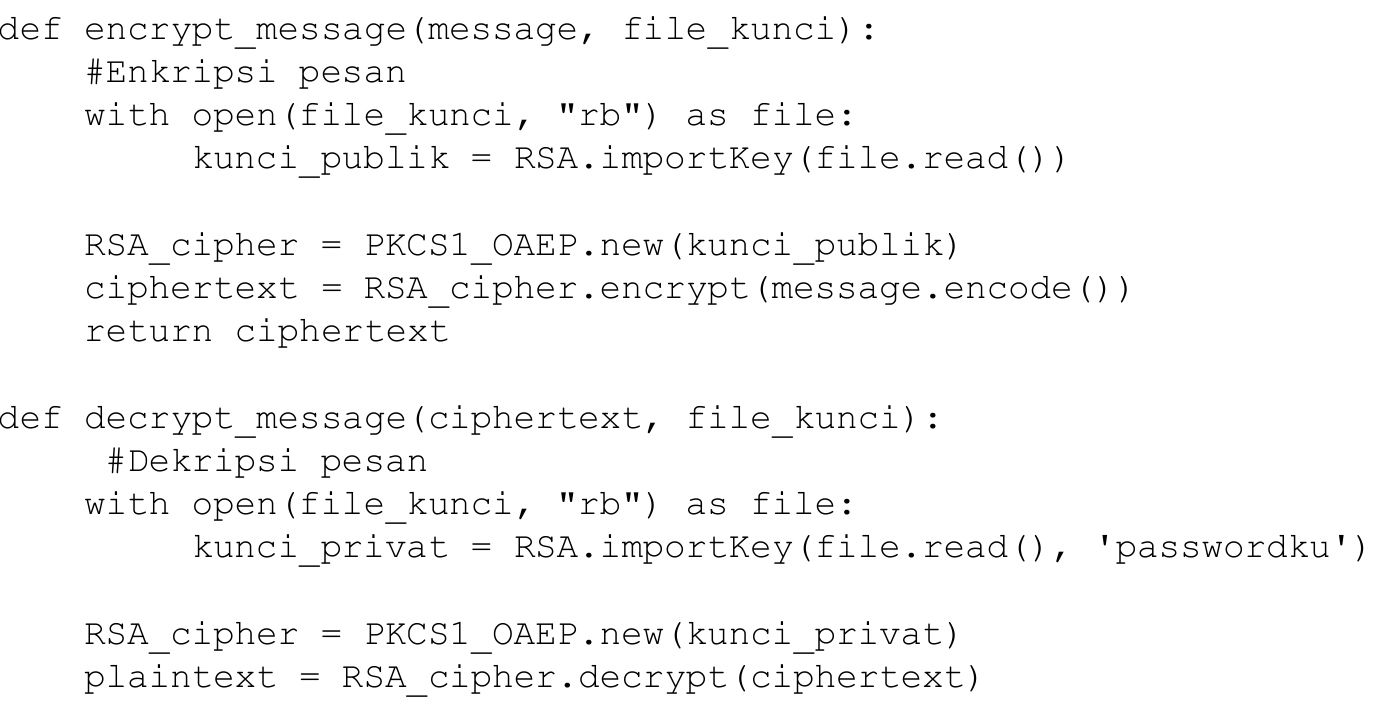
\includegraphics[width=151.20mm,height=193.05mm]{../../images/llm/page_043_img_01.png}%
\end{textblock*}

\end{document}
